\section{Distributed MSI}
\label{sec:DistributedMsi}

We will take the protocol designer's perspective, and first describe what the
designer has to specify to create a distributed protocol.

Each cache can only read and write its local state. A cache maintains a shadow
 of all its children's states in the form of a directory. The designer can
always assume that the state of an actual child is what is given in the
directory. The directory entry of address $a$ for $this$' child $c$ is denoted
using $this.dir[c][a]$.

The designer has to specify the handlers for \uReq{} and \dReq{}. In the
following, we assume that the cache whose handler the designer is writing is
$this$ and the relevant address is $a$.

In order to read a child's state, the designer simply reads the state of the
directory for that child. But to modify the state of child $c$ to $x$, the
designer specifies a command \send{} \Req{this}{c}{a}{x}, followed by \receive{}
\Resp{c}{this}{a}{y}. Command \send{} \Req{this}{c}{a}{x} can be called only when $x
< this.dir[c][a]$. $y$ denotes a free variable which gets filled with the value of
the state $c$ has changed to. $y$ is guaranteed to be $\le x$. $this.dir[c][a]$
should be updated with this value.

In order to read the data of another node $n$ (parent or child),
the designer issues the command \receive{} \Data{this}{n}{a}{d}, where $d$ is a free
variable that gets filled with the data. To write the data into address $a$ of
another node $n$ (parent or child), the designer issues the command \send{}
\Data{this}{n}{a}{this.data[a]}.

In order to upgrade the state of $this$ to $x$, the designer has to
specify the command \send{} \Req{this}{p}{a}{x} followed by \receive{}
\Resp{p}{this}{a}{y}. Command \send{} \Req{this}{p}{a}{x} can be called only when $x
> this.state[x]$. $y$ denotes a free variable which gets filled with the value of
the state $this$ should be upgraded to. $y$ is guaranteed to be $\ge x$.

Using these commands, the designer can now easily specify a distributed MSI
protocol, by specifying the methods \uReq{} and \dReq{}. Three other
obligations to take care of:
\begin{enumerate}
\item Handler \uReq{}($c, a, x$) can be called even if $x \ge
this.dir[c]$. In this case, it should be dropped.
\item Handler \dReq{}($p, a, x$) can be called even if $x \le
this.state[a]$. In this case, it should be dropped.
\item A new handler, \dRespL{}($c, a, x$), where $c$ is a child of cache $this$,
should be provided, and this informs $this$ that $c$ has changed its state to
$x$.
\end{enumerate}

Using the above set of rules, the designer can specify the distributed MSI protocol as shown in
Figure \ref{realistic}. Handlers \uReq{} and \dReq{} are exactly the same as
shown in Figure \ref{msi-template}, except that whenever the state of a child
$c'$ is read, it should be replaced syntactically by $this.dir[c'][a]$.

\begin{figure}
\small
\begin{algorithmic}
\Proc {\dRespL}{$c , a, x$}
  \If {$isModified(this.dir[c][a])$}
    \State \receive{} \Data{c}{this}{a}{d};
    \State $this.data[a] \gets d$;
  \EndIf
\EndProc
\end{algorithmic}
\caption{Handling an voluntary response message from a child $c$, sent if the
child evicts line $a$ and downgrades the line to $x$}
\label{msi-unsolicited}
\end{figure}

\begin{figure}
\small

\begin{algorithmic}
\State // Upgrading $this$ by sending request to parent and getting a response
\Proc {\uReqL}{$p, a, x$}
  \If {$this$ is LLC \&\& $this.state[a] = I$}
    \State \send{} \Req{this}{Memory}{a}{M};
    \State \receive{} \Data{Memory}{this}{a}{d};
    \State $this.data[a] \gets d$;
    \State $this.state[a] \gets M$;
  \Else
  \State \send{} \Req{this}{p}{a}{x};
  \State \receive{} \Resp{p}{this}{a}{z};
  \If {$this.state[a] = I$}
    \State \receive{} \Data{p}{this}{a}{d};
    \State $this.data[a] \gets d$;
  \EndIf
  \State $this.state[a] \gets z$;
  \EndIf
\EndProc
\State // Downgrading $this$' child by sending request to child and getting a
response
\Proc {\dReqL}{$c, a, x$}
  \State \send{} \Req{this}{c}{a}{x};
  \While {$this.dir[c][a] > x$}
  \State \receive{} \Resp{c}{this}{a}{z};
  \If {$isModified(this.dir[c][a])$}
    \State \receive{} \Data{c}{this}{a}{d};
    \State $this.data[a] \gets d$;
  \EndIf
  \State $this.dir[c][a] \gets z$;
  \EndWhile
\EndProc
\State // $this$ finally upgrading the directory state of its child and sending
a response to its child
\Proc {\uResp}{$c, a, x$}
  \State \textbf{if} ($this.dir[c][a] = I$)
  \State \;\;\;\; \send{} \Data{this}{c}{a}{this.data[a]};
  \State $this.dir[c][a] \gets x$;
\EndProc
\State // $this$ finally downgrading its state and sending a response to its
parent
\Proc {\dResp}{$p, a, x$}
  \State \textbf{if} ($isModified(this.state[a])$)
  \State \;\;\;\; \send{} \Data{this}{p}{a}{this.data[a]};
  \State $this.state[a] \gets x$;
\EndProc
\end{algorithmic}
\caption{Distributed MSI protocol. In all the methods $p$ is the parent of
$this$, $c$ is a child of $this$, and the methods work on address $a$ to change
its state (or directory) to $x$. This function only shows the auxiliary
functions and the handler for voluntary responses from children. The handler
for requests are exactly the same as in Figure \ref{msi-template}, with every
occurrence of $c'.state[a]$ replaced by $this.dir[c'][a]$}
\label{realistic}
\end{figure}

Even though the designer only specifies the distributed protocol in the manner we have
written in Figure \ref{realistic}, we automatically
create a correct implementation of the cache controller from this
specification.  The commands \send{} and \receive{} get translated into
appropriate request and response messages which get sent to or received from the respective
nodes, and they invoke the corresponding message handlers. Note that in the final
implementation, sending of a message blocks if there is no space in the output
channel and receiving of a message blocks if there is no message available for
reception, though the designer is oblivious to this fact. We will describe how
the specification is translated to an actual implementation, and show why the
implementation is correct.

\subsection{Caches as a system executing suspensive threads}
The behavior of each cache node can be best described as a system of suspensive
threads. These correspond to Miss Status Handling Register (MSHRs) in an actual
implementation. A scheduler creates and schedules threads within the cache.  A
new thread is created whenever a new message arrives in the input channel, and
no other thread is executing. When a thread is executing a \send{} command, then
an actual message is created and sent to the appropriate cache. The thread then
goes into a suspend state till it receives a response message indicating that
the requested state change has taken place. In this case, the suspended thread is
woken up by the scheduler to perform the rest of its actions. Once all of its
actions are complete, a thread dies, and its resources are freed.

Each request goes through several stages of processing in a cache (as shown in
Figure \ref{msi-template}). This is the reason for using the vocabulary of
threads instead of MSHRs -- a thread makes the processing stage a particular
request is currently in, implicit.

Now that we have established the vocabulary of threads, we will proceed to
describe the requirements that a network should guarantee in order to make such
an implementation possible. We will also show the scheduling algorithm that we
generate.

\subsection{Message ordering requirements}
\floatstyle{boxed}
\restylefloat{figure}

%The basic ordering requirement is that responses should not overtake each other
%when they are sent from the same source to the same destination. Similarly,
%requests should not overtake responses from the same source to the same
%destination.

\begin{figure}\small
\begin{requirement}
An incoming response for an address $a$ from a child $c$ should not be
received before another incoming response from the same $c$ and the
same $a$ sent earlier has been received\label{cRespFifo}
\end{requirement}
\begin{requirement}
An incoming request for an address $a$ from a source $n$ should not be
received before another incoming response from the same $n$ and the
same $a$ sent earlier has been received\label{reqNoOvertakeResp}
\end{requirement}
\caption{Ordering requirements}
\label{order}
\end{figure}

Figure \ref{order} gives the exact ordering
requirements between messages transmitted between the caches.

We will illustrate the need for Requirements \ref{cRespFifo} and
\ref{reqNoOvertakeResp} using a 2-level cache hierarchy with two L1 caches $c_1$ and
$c_2$, and one shared L2 cache $p$. Each core can have several outstanding
memory requests.

\floatstyle{plain}
\restylefloat{figure}
\begin{figure}
\centering
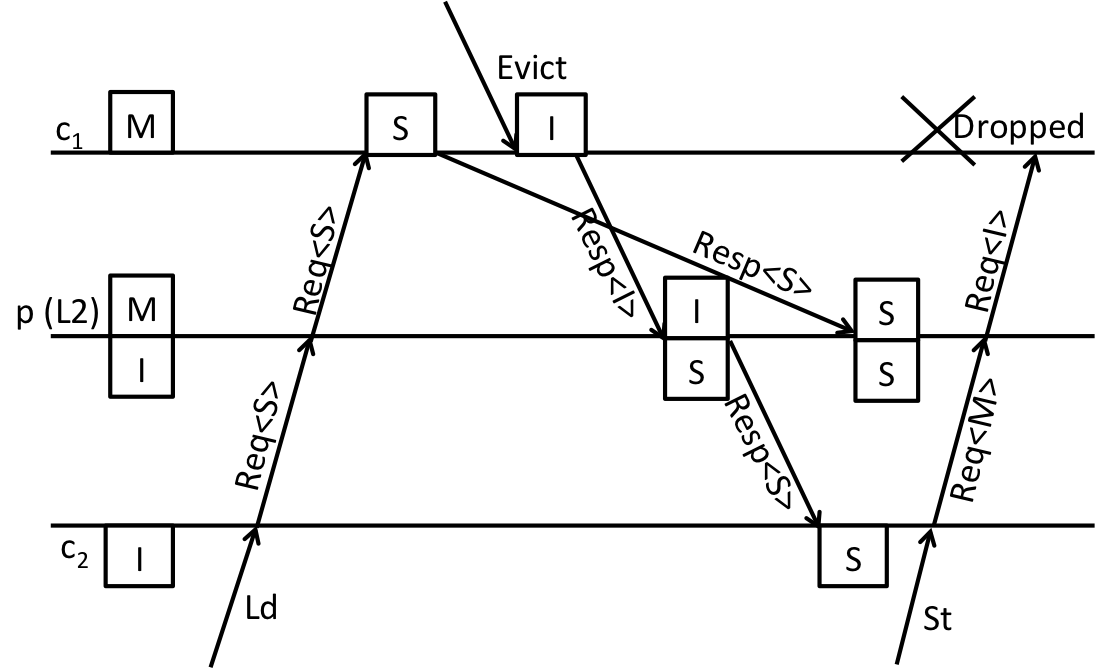
\includegraphics[scale=0.4]{complicated}
\caption{Effect of violating Requirement \ref{cRespFifo} (order between responses)}
\label{complicated}
\end{figure}
\floatstyle{boxed}
\restylefloat{figure}

Let's say $c_1.state[a] = p.dir[c_1][a] = M$, $c_2.state[a] = p.dir[c_2][a] =
I$. $c_2$ gets a load request from its processor for address $a$ and sends an
upgrade request to $p$. $p$ sends a downgrade-to-$S$ request to $c_1$. $c_1$
receives the downgrade-to-$S$ request and downgrades to $S$, sending a downgrade
response to $p$. $c_1$ decides to evict address $a$ to make room for another
address $a'$, because of a request from the core for $a'$ not present in $c_1$.
$c_1$ sends a downgrade-to-$I$ response to $p$. Let's say the second downgrade
to $I$ response reaches $p$ first, violating Requirement \ref{cRespFifo}. $p$
sends an upgrade-to-$S$ response to $c_2$. $c_2$ receives the upgrade response
and changes state to $S$. $p$ then receives the second downgrade-to-$S$ response
from $c_1$, changing its $p.dir[c_1][a]$ to $S$. $c_2$ sends an upgrade-to-$M$
request to $p$ because of a store from its core for $a$. $p$ will send a
downgrade-to-$I$ request to $c_1$, but $c_1$ drops the request as seen in
procedure \dReq{} in Figure \ref{realistic}. So $p$ will never receive a
response from $c_1$ leading to a deadlock. This is illustrated in Figure
\ref{complicated}. In the figure, the timeline moves from left to right.
Whenever the state of the directory or the cache changes, we show the new state.
Messages are shown using arrows from the source to the destination, moving
across time.

\floatstyle{plain}
\restylefloat{figure}
\begin{figure}
\centering
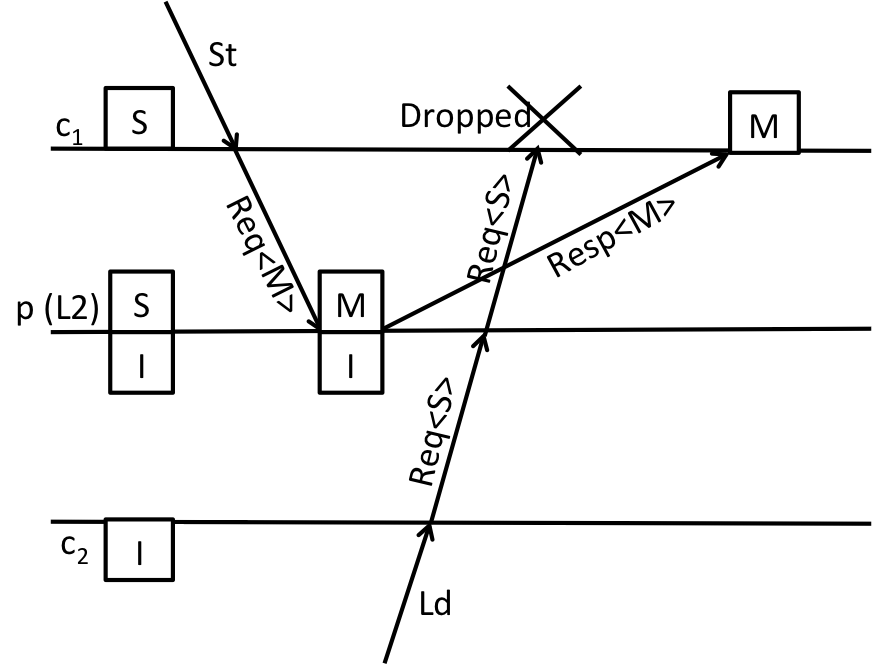
\includegraphics[scale=0.4]{lessComplicated}
\caption{Effect of violating Requirement \ref{reqNoOvertakeResp} (requests overtaking responses)}
\label{lessComplicated}
\end{figure}
\floatstyle{boxed}
\restylefloat{figure}

Consider another scenario starting with $c_1.state[a] = p.dir[c_1][a] = S$ and
$c_2.state[a] = p.dir[c_2][a] = I$. $c_1$ receives a store request and sends an
upgrade-to-$M$ request to $p$. $p$ sends back an upgrade-to-$M$ response to
$c_1$. $c_2$ gets a load request for address $a$ and sends an upgrade-to-$S$
request to $p$. $p$ sends a request to $S$ to $c_1$. Suppose Requirement
\ref{reqNoOvertakeResp} is violated and the request to $S$ reaches $c_1$ before
the response to $M$. $c_1$ will drop the request since its already in state $S$,
and so $p$ will never get a response leading to a deadlock. This is illustrated
in Figure \ref{lessComplicated}.

These scenarios show that these ordering requirements are indeed necessary for a
correct cache coherence protocol.

\subsection{Resource requirements and blocking restrictions}

\begin{figure}\small
\begin{requirement}
At a cache node, an incoming request from the parent should not be blocked by any
incoming request from its children.\label{cReqNoBlockPReq}
\end{requirement}
\begin{requirement}
At a cache node, an incoming response from any of its children should not
be blocked by any incoming requests.\label{reqNoBlockResp}
\end{requirement}
\begin{requirement}
At a cache node, an incoming response for address $a$ from its parent should not be blocked by
an incoming request from its child for address $a$. \label{reqBlockResp2}
\end{requirement}
\caption{Blocking restrictions}
\label{blocking}
\end{figure}

Figure \ref{blocking} shows the restrictions that the input channels should
obey with respect to an incoming message blocking other incoming messages.

\begin{figure}\small
\begin{requirement}
Each cache node has at least one dedicated thread resource for handling only messages
(requests or responses) from the parent\label{dedicate1}
\end{requirement}
\begin{requirement}
Each cache node has at least one dedicated thread resource for handling only responses
(from children or from the parent)\label{dedicate2}
\end{requirement}
\begin{requirement}
Each cache node has at least three thread resources\label{dedicate3}
\end{requirement}
\caption{Dedicated resources in a cache node}
\label{dedicated}
\end{figure}

Figure \ref{dedicated} shows the minimum number of thread resources that should
be present in each cache node. Lack of required thread resouces leads to the same
kind of deadlock scenarios as incorrect blocking does. This is illustrated in the
following:

Let's say both $c_1.state[a] = p.dir[c_1][a] = S$ and $c_2.state[a] =
p.dir[c_2][a] = S$. Both $c_1$ and $c_2$ get store requests from the processor
for address $a$, and they send upgrade-to-$M$ requests to $p$.  $p$ receives the
request from $c_2$ first. $p$ sends a downgrade-to-$I$ request to $c1$.

\floatstyle{plain}
\restylefloat{figure}
\begin{figure}
\centering
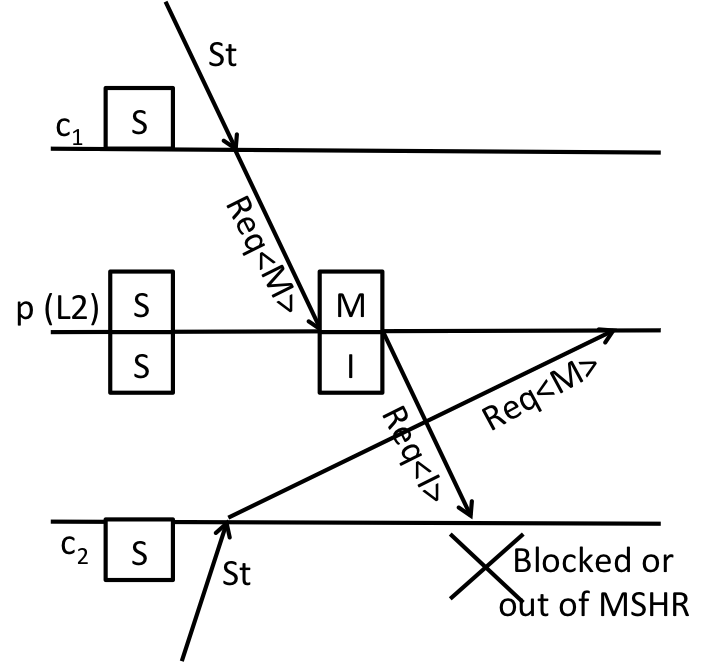
\includegraphics[scale=0.4]{unknown}
\caption{Effect of violating Requirement \ref{cReqNoBlockPReq} (requests blocking responses from parent)}
\label{unknown}
\end{figure}
\floatstyle{boxed}
\restylefloat{figure}

Let's say Requirement \ref{cReqNoBlockPReq} is not held, and instead some request
from the core is blocking $c_1$ from receiving the request. $c_1$ will never
respond back to $p$. But $p$ will be waiting in procedure \dReqL{}, and will
never start handling the request from $c_1$. This will create a deadlock.  The
same deadlock is also created when $c_1$ is out of thread resources to create a
thread to handle the downgrade request from $p$ (violating Requirement
\ref{dedicate1}). Figure \ref{unknown} depicts this scenario.

Let's extend this scenario further. Instead of violating Requirements
\ref{cReqNoBlockPReq} or \ref{dedicate1}, let $c_1$
send a downgrade-to-$I$ response to $p$. Let's instead assume that Requirement
\ref{reqNoBlockResp} is violated in $p$. So, the downgrade-to-$I$ response from
$c_1$ is not received by $p$, leading to the same deadlock. This is the same if
Requirement \ref{dedicate2} is violated and $p$ is out of thread resources to
create a thread to handle the downgrade response.

The need for Requirement \ref{dedicate3} can be shown easily. Let's say that a
cache has exactly 2 thread resources, one for handling messages from parents,
and one for handling responses from either the parent or the children. Now, if
it receives a request from one of its children, it can not use either of the
thread resources. Thus, at least one more thread resource is needed for
handling requests from children. This thread resource can also be used for
handling other types of incoming message.

\subsection{Scheduler requirements}

We will now list the requirements that a scheduler must obey to give the
illusion of non-suspensive threads and avoid deadlocks.

\begin{figure}\small
\begin{requirement}
$p$ can not receive a request \Req{c}{p}{a}{x} from $c$, where $p = c.parent$,
if either
\begin{enumerate}
\item address $a$ has been chosen for eviction by some thread and that thread
has not yet replaced $a$, or
\item a thread in $p$ is handling a request for address
$a$ from any source
\end{enumerate}
\label{pHandleReq}
\end{requirement}
\begin{requirement}
$c$ can not receive a request \Req{p}{c}{a}{x} from $p$, where $p = c.parent$,
if either
\begin{enumerate}
\item address $a$ has been chosen for eviction by some thread and that thread
has not yet replaced $a$, or
\item a thread in $c$ is handling a request for address
$a$ from $p$, or
\item a thread in $c$ is handling a request for address
$a$ from one of $c$'s children $c'$, but that thread is not waiting for a
response from $p$
\end{enumerate}
\label{cHandleReq}
\end{requirement}
\caption{Requirements for receiving a request (used by the scheduler)}\label{recvReq}
\label{}
\end{figure}

\begin{figure}\small
\begin{requirement}
Address $a$ present in cache node $c$ can not be chosen for eviction by a thread
executing in $c$ if either
\begin{enumerate}
\item address $a$ has been chosen for eviction by some thread and that thread
has not yet replaced $a$, or
\item a thread in $c$ is handling a request for address
$a$ from any source
\end{enumerate}\label{evict}
\caption{Requirements for suspending a thread during choosing an address for eviction}
\end{requirement}
\end{figure}

Requirements \ref{pHandleReq}, \ref{cHandleReq} and \ref{evict} are needed
because once a thread has finished up-to a point in its execution, it can not
re-execute that portion. For instance, consider a thread handling an upgrade
request from a child. Let's say thread $t$ has progressed to the point where it
is simply waiting to send an upgrade response to the child. Now, if the line
gets evicted because it was chosen for replacement, or it got downgraded by the
parent, then thread $t$ can not re-execute its procedure again. To prevent this,
only one thread is allowed to operate on a particular address, except in the
case of downgrade requests from the parent. In this case, a thread is created to
handle the downgrade request from the parent even if there is another thread
handling a request for the same address from a child, if the latter thread is
just waiting for a response from the parent. This is done to avoid deadlocks
like the ones shown in Figure \ref{unknown}.

\begin{figure}\small
\begin{requirement}
Starvation-freedom: A thread that keeps becoming ready to execute will
eventually be scheduled to execute.\label{starvation}
\end{requirement}
\end{figure}

Local starvation-freedom is required in each cache node. If a cache node never
executes a particular suspended thread, even if it keeps getting ready to
execute, then the thread will not progress, leading to a deadlock.

A scheduler can be implemented as described in Figure \ref{scheduler}, obeying
Requirements \ref{pHandleReq} and \ref{cHandleReq}. It should perform some form of
fair arbiration among its suspended threads to avoid starvation (Requirement
\ref{starvation}).

\newcommand{\lWhile}{\textbf{while}}
\newcommand{\lIf}{\textbf{if}}
\newcommand{\lElsIf}{\textbf{else if}}
\newcommand{\lElse}{\textbf{else}}

\floatstyle{plain}
\restylefloat{figure}

\begin{figure}
\small
\begin{boxedminipage}{\linewidth}
\begin{alltt}
\normalfont
\lWhile{} (\(True\)) \bopen
      \lIf (\Resp{c}{n}{a}{x} is in the input channel,
            where \(n = c.parent\)) \bopen
            \lIf (suspended thread \(t\) is waiting for 
                 a response from \(c\) for address \(a\)) \bopen
                   \resume{} \(t\);
            \bclose \lElse \bopen
                   \receive{} \Resp{c}{n}{a}{x};
                   \start{} \dRespL(\(c, n, a, x\));
            \bclose
      \bclose \lElsIf (\Resp{p}{n}{a}{x} is in the input channel,
            where \(p = n.parent\)) \bopen
                   // There must be a suspended thread \(t\)
                   waiting for a response from \(p\) for address \(a\)
                   \resume{} \(t\);
            \bclose
      \bclose \lElsIf (\Req{c}{n}{a}{x} is in the input channel,
                     where \(n = c.parent\)) \bopen
             \lIf (Local-Property \ref{pHandleReq} is satisfied) \bopen
                   \receive{} \Req{c}{n}{a}{x};
                   \start{} \uReq(\(c, n, a, x\));
             \bclose
      \bclose \lElsIf (\Req{p}{n}{a}{x} is in the input channel,
                  where \(p = n.parent\)) \bopen
             \lIf (Local-Property \ref{cHandleReq} is satisfied) \bopen
                   \receive{} \Req{p}{n}{a}{x};
                   \start{} \dReq(\(p, n, a, x\));
             \bclose
      \bclose \lElsIf (suspended thread \(t\) is ready to execute) 
             \resume{} \(t\);
\bclose
\end{alltt}
\end{boxedminipage}
\caption{Implementation of a scheduler for cache node $n$}
\label{scheduler}
\end{figure}
